\chapter{Разработка рациональной конструкции БПЛА}

В этой главе рассматривается задача многодисциплинарного проектирования конструкции гипотетического БПЛА с крылом большого удлинения и с искривленной конструкцией центроплана.  Основной целью данной задачи является минимизация веса конструкции БПЛА при обеспечении необходимой прочности и жесткости и удовлетворении ограничениям на проектные параметры. При разработке конструкции учитывалась необходимость того, чтобы некоторые ограничения на проектные параметры могли быть в дальнейшем легко изменены. Гипотетический БПЛА по многим базовым проектным параметрам имеет сходство с "БПЛА-ЦАГИ", разработанным в НИО-10 ЦАГИ.


\section{Особенности проектирования конструкции БПЛА}


В работе был рассмотрен ?вопрос проектировки? беспилотного летательного аппарата (БПЛА), предназаченного для длительного ($\approx24$~часа без дозаправки) барражирования в целях мониторинга и разведки (ограничения по режимам полета представлены на Рис.\ref{fig:ModeOfFlight}). В связи с этим к БПЛА были предъявлены высокие требования по малозаметности и аэродинамическому качеству. 


За основу была взята разработанная в ЦАГИ модель БПЛА, хорошо отвечающая требованиям аэродинамического качества и малозаметности. Вид фюзеляжа выбранной модели показан на Рис.\ref{fig:BPLA_TSAGI}.
 

%Возможно, вставить пункт с геометрическими ограничениями
  
  



\begin{figure}[ht]
\centering
\includegraphics[width=1\textwidth]{BPS_Catia_Full}
\caption{Вид модели БПЛА-ЦАГИ}
\label{fig:BPLA_TSAGI}
\end{figure}

Данная модель выполнена по схеме ``бесхвостка'' с крылом большого удлинения, интегрированным с фюзеляжем. 

Для интеграции двигателя с воздухозаборником в конструкцию данной модели в конструкции используется изогнутый центроплан. Использование такой формы центроплана сопряжено с возможным возникновением проблем обеспечения прочности в связи с большими изгибающими моментами в нём. 

Использование такого центроплана может существенно ухудшить компоновку и весовую эффективность БПЛА по сравнению с использованием прямого центроплана. Исследований центропланов такой формы ранее не проводилось. В данной работе проведен анализ возможных ухудшений весовой эффективности. 
 
%очевидно, что волнообразный центроплан может иметь напряжные вопросы с обеспечением прочности, т.к. такие центропланы в такой размерности не использовались, довольно нагружены. Сказать про компоновку, нарисовать её (общие вещи).

%с самого начала пишем, какие проблемы. Так сделали, такая компоновка, но у неё такие-то проблемы след волнообразный центроплан

%дальше: это может существенно ухудшить компоновку и весовую эффективность по сравнению с прямым центропланом. Цель работы - оценить возможные ухудшения. 

% и уже для того, чтобы оценить: следующий параграф 

Для оценки возможных ухудшений весовой эффективности и компоновки была поставлена задача построения расчетной модели данного БПЛА и прочностного анализа созданной модели. 
При построении модели необходимо было учесть ее дальнейшую модификацию, позволяющую варьировать форму внешних аэродинамических обводов. В бакалаврской работе форма внешних аэродинамических обводов постоянны. Также постоянными считаются нагрузки на конструкцию (см.Раздел \ref{sec:externalLoads}). 

%В бакалаврской работе будем рассматривать только те обводы, которые есть в этой модели. И целью работы будет оценка потерь из-за такого центроплана (в прочности)

 
  
  

%Не забыть про то, что мы также хотим менять аэродинамику
%Требования: БПЛА, полет на таких-то высотах, столько-то. Весовая сводка такая-то, максимальные перегрузки, коэффициент запаса, аэродинамика. Ограничения - малозаметность, вес, пожаробезопасность отсека двигателя. 
%




\section{Компоновочная схема}
На рисунках 
\ref{fig:BPS_Catia_Top}--\ref{fig:BPS_Catia} показана модель гипотетической конструкции БПЛА.
%\begin{itemize}
%\item размах крыльев: $\approx37\text{м}$
%\item высота фюзеляжа: 1.7м
%\item длина фюзеляжа: 7м
%\end{itemize}


\begin{figure}[H]
\centering
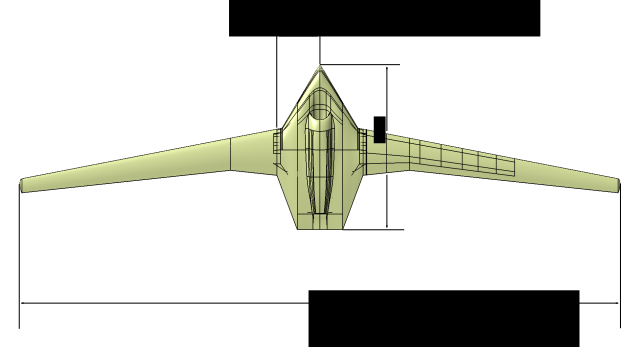
\includegraphics[width=0.8\textwidth]{BPS_Catia_Top}
\caption{Вид сверху}
\label{fig:BPS_Catia_Top}
\end{figure}
%На рисунках проставить размеры

Как видно из рисунков для данной компоновочной схемы используется крыло большого удлинения. Из рисунка \ref{fig:BPS_Catia_WithoutSkin}, на котором представлена базовая конструктивно-силовая схема БПЛА, можно видеть, как происходит интеграция корпуса фюзеляжа, крыла и двигателя. 

\begin{figure}[H]
\centering
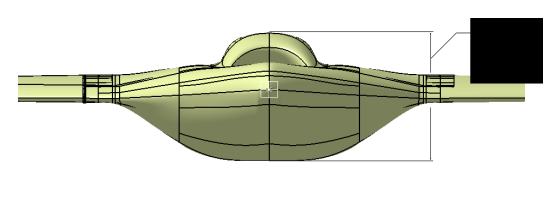
\includegraphics[width=0.8\textwidth]{BPS_Catia_Front}
\caption{Вид фюзеляжа спереди}
\label{fig:BPS_Catia_Front}
\end{figure}




\begin{figure}[H]
\centering
\includegraphics[width=0.8\textwidth]{BPS_Catia}
\caption{Вид фюзеляжа в изометрии}
\label{fig:BPS_Catia}
\end{figure}

%\begin{figure}[H]
%\centering
%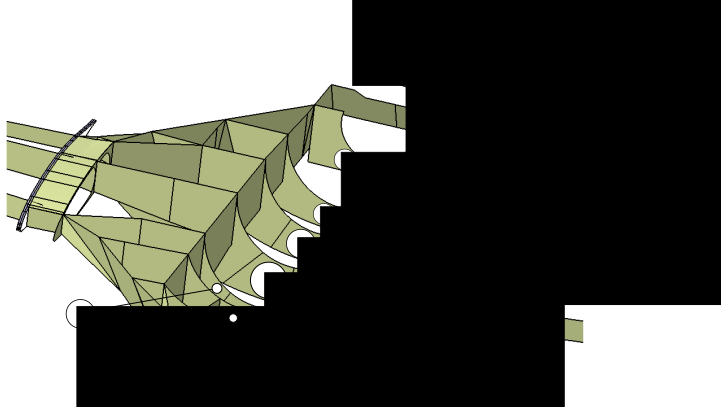
\includegraphics[width=0.8\textwidth]{BPS_Catia_WithoutSkin}
%\caption{Вид фюзеляжа со снятой обшивкой}
%\label{fig:BPS_Catia_WithoutSkin}
%\end{figure}

\begin{figure}[H]
\centering
\def\svgwidth{0.9\textwidth}
\input{figures/BPS_Catia_WithoutSkin.pdf_tex}
\caption{Вид фюзеляжа со снятой обшивкой с указанием узлов крепления шасси и двигателя}
\label{fig:BPS_Catia_WithoutSkin}
\end{figure}

Из рисунка видно, что двигатель с воздухозаборником значительно утоплены и находятся практически в середине фюзеляжа. Как уже отмечалось выше, эта особенность позволяет значительно улучшить малозаметность и аэродинамическое качество самолета (ссылка на отчет), но приводит к необходимости формировать искривленный центроплан. 

Формирование искривленного центроплана создает дополнительные проблемы из-за большой величины изгибающего момента в корне крыла. Еще одной проблемой обеспечения прочности корпуса БПЛА является высокая чувствительность параметров управляемости БПЛА от жесткостных характеристик корпуса и особенно зоны стыка крыла с центропланом, где расположены узлы крепления стоек основного шасси. Очевидно, что для решения проектировочной задачи необходимо проведение комплексных исследований прочности данной конструкции включая анализ прочности, устойчивости и управляемости. 

В данной схеме используется только горизонтальное оперение: руль высоты. Механизация крыла состоит из расщепляющихся элеронов на концах крыльев, элевонов и интерцепторов. В качестве тяги используется один реактивный двигатель, установленный в канале воздухозаборника. Места креплений стоек и замков шасси, расположение двигателя и узлов его крепления показаны на Рис. \ref{fig:BPS_Catia_Top_WithoutSkin}. 


\begin{figure}[H]
\centering
\def\svgwidth{0.9\textwidth}
\input{figures/BPS_Catia_Top_WithoutSkin.pdf_tex}
\caption{Вид сверху без обшивки с указанием узлов крепления шасси и двигателя}
\label{fig:BPS_Catia_Top_WithoutSkin}
\end{figure}

Отсеки фюзеляжа делятся на несколько групп по назначению. Распределение отсеков фюзеляжа по назначению представлено на Рис.\ref{fig:BPS_Catia_Top_PartRoles}. 

На рис.\ref{fig:BPS_Catia_Top_PartRoles} схематически показаны основные отсеки конструкции БПЛА. 

\begin{figure}[H]
\centering
\def\svgwidth{0.9\textwidth}
\input{figures/BPS_Catia_Top_PartRoles.pdf_tex}
\caption{Вид сверху с обозначением роли отсеков}
\label{fig:BPS_Catia_Top_PartRoles}
\end{figure}




%Пока кратко: Крыло большого удлинения интегрировано с фюзеляжем. Двигатель утоплен в конструкцию, подвод воздухозаборника, сопло над горизонтальным оперением. В передней части фюзеляжа расположены отсеки с БРЭО, отсеки с топливом, отсек под переднее шасси. 
% задней части фюзеляжа пара отсеков под топливо, отсеки под БРЭО, шассийные отсеки, шасси крепится на стыке крыла с фюзеляжем. 







%Описываем полностью всю конструкцию. Показываем много разных картинок. 	

\section{Внешние нагрузки}
\label{sec:externalLoads}
Внешние расчетные нагрузки на гипотетическую конструкцию БПЛА были сформированы на основе результатов проведенных в ЦАГИ исследований \cite{BPS_TSAGI} по анализу внешних нагрузок на конструкцию БПЛА-ЦАГИ. Для предварительных расчетов прочности гипотетической конструкции БПЛА в рамках данной работы использовался один расчетный случай нагружения А, который оказался наиболее критичным для основных силовых элементов центроплана и зоны стыка крыла и фюзеляжа. 

Для силовых элементов конструкции носовой и концевой части фюзеляжа были сформированы еще два случая нагружения. 


Для основного случая нагружения основные параметры, формирующие внешнее нагружение следующие: нормальная перегрузка $n_y = 2.97$, $M = 0.4$, скоростной напор $q = 503 \text{кгс}/\text{м}^2$, высота полета $H = 6.5\text{км}$. Нагрузки на гипотетическую конструкцию БПЛА получены на основе пересчета из работы \cite{BPS}.

Эпюры аэродинамических нагрузок на крыло представлены на Рис.\ref{fig:BendingMoments},\ref{fig:RotatingMoments}.


\begin{figure}[H]
\centering
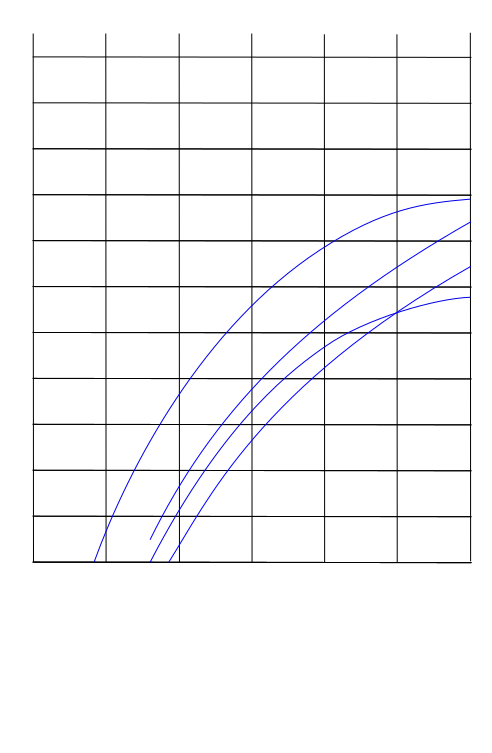
\includegraphics{HeightGraph}
\caption{Ограничения на расчетные режимы полета (случай А)}
\label{fig:ModeOfFlight}
\end{figure}


%уточнить, что где, подписать адекватно. Понять! Обозначить случай, который считаем. 

%\begin{figure}[H]
%\centering
%\def\svgwidth{0.9\textwidth}
%\input{figures/Heights.pdf_tex}
%\caption{Ограничения на режимы полета}
%\label{fig:ModeOfFlight}
%\end{figure}


\begin{figure}[H]
\centering
\def\svgwidth{0.9\textwidth}
\input{figures/BendingMoments.pdf_tex}
\caption{Эпюра изгибающих моментов}
\label{fig:BendingMoments}
\end{figure}


%\begin{figure}[H]
%\centering
%\def\svgwidth{0.9\textwidth}
%\input{figures/BendingAndRotatingMoments.pdf_tex}
%\caption{Эпюры изгибающих и крутящих моментов}
%\label{fig:BendingAndRotatingMoments}
%\end{figure}

%\begin{figure}[H]
%\centering
%\def\svgwidth{0.9\textwidth}
%\input{figures/CuttingForces.pdf_tex}
%\caption{Эпюра перерезывающих сил}
%\label{fig:CuttingForces}
%\end{figure}

%\begin{figure}[H]
%\centering
%\def\svgwidth{0.9\textwidth}
%\input{figures/DistributedLoad.pdf_tex}
%\caption{Эпюра погонной нагрузки}
%\label{fig:DistributedLoad}
%\end{figure}

\begin{figure}[H]
\centering
\def\svgwidth{0.9\textwidth}
\input{figures/RotatingMoments.pdf_tex}
\caption{Эпюра крутящих моментов}
\label{fig:RotatingMoments}
\end{figure}


Как видно из имеющихся данных (Рис.\ref{fig:BendingMoments}--\ref{fig:RotatingMoments}), влияние кручения на крыло невелико по сравнению с изгибом. В связи с этим в дальнейшем в работе при решении некоторых модельных задач будет целесообразно пренебрегать кручением крыла, рассматривая только изгибные деформации. 




\section{Расчетные прочностные модели}
%\section{Создание конечно-элементной модели проектируемого самолета}

В ходе работы были исследованы вопросы построения проектировочной модели БПЛА с крылом большого удлинения и несущим фюзеляжем. При помощи программного комплекса ``Conver'' (см. раздел \ref{sec:Conver}), исходя из взятой за основу концептуальной модели, была создана МКЭ-модель проектируемого БПЛА с исключенной верхней частью воздухозаборника, не несущей в себе силовых элементов. 

%\begin{figure}[ht]
%\centering
%\includegraphics[width=0.8\textwidth]{BPLAfullModel}
%\caption{МКЭ-модель проектируемого БПЛА без верхней части}
%\label{fig:BPLAfullModel}
%\end{figure}

\subsection{Требования к прочностной модели}

К прочностной модели предъявляются следующие требования:

\begin{enumerate}
\item оперативность построения модели
\item подробность модели
\item надежность анализа
\item возможность модификации 
\item рациональный выбор конечно-элементной сетки
\end{enumerate}

%Выбор базового комплекса
\subsection{Выбор базового комплекса}
Учитывая представленные выше требования к модели, для построения моделей в работе был использован программный комплекс ``Conver'', разработанный в НИО-3 ЦАГИ. 
% в описании конвера расписывать, чем он нам подходит
%\subsection{Программный комплекс ``Conver''}
\label{sec:Conver}

Для построения описанных выше моделей использовался разработанный в ЦАГИ программный комплекс ``Conver''. Его использование позволило многократно сократить время построения каждой модели. 

%\subsection{Описание комплекса}
Комплекс представляет собой многоуровневую среду для автоматизированного проектирования и оптимизации ЛА. Комплекс делится на 4 уровня по степени детализации:



\begin{figure}[ht]
\centering
\includegraphics[width=0.6\textwidth]{ConverCircle} 
\caption{Принципиальная схема четырехуровневого проектирования}
\end{figure}



\begin{itemize}
\item Уровень 1: расчёт аэродинамических нагрузок и аэродинамических характеристик; 
\item Уровень 2: расчёт инерционных нагрузок, формирование случаев нагружения, решение задач статической и динамической аэроупругости, анализ веса конструкции планера;
\item Уровень 3: расчёт местной и общей устойчивости, анализ закритического состояния отдельных элементов конструкции, расчёт нелинейного НДС панелей гермокабины, расчет несущей способности элементов конструкции;
\item Уровень 4: расчёт общего НДС конструкции ЛА, определение запасов прочности, определение остаточной прочности, расчет длительной прочности.
\end{itemize}

Основные особенности программного комплекса:

\begin{enumerate}
\item Эффективное проведение параметрических исследований для различных конструкций планера, что позволяет минимизировать временные затраты и снизить трудоёмкость всего процесса;
\item Обеспечение более высокого качественного уровня параметрических исследований на начальной стадии проектирования за счёт автоматизированного создания полноразмерных моделей конструкции ЛА и автоматизации процесса анализа результатов исследований;
\item Оперативная оценка веса конструкций летательных аппаратов с учётом технологических ограничений при автоматическом использовании специализированных баз данных поправочных технологических коэффициентов.
\end{enumerate}

%Нарисовать блок-схему взаимодействия nastran patran conver расчетная модель автокад аэродинамика


%\section{Программный комплекс ``Conver''}

\subsection{Описание комплекса}
Комплекс представляет собой многоуровневую среду для автоматизированного проектирования и оптимизации ЛА. Комплекс делится на 4 уровня по степени детализации:



\begin{figure}[ht]
\centering
\includegraphics[width=0.6\textwidth]{ConverCircle} 
\caption{Принципиальная схема четырехуровневого проектирования}
\end{figure}



\begin{itemize}
\item Уровень 1: расчёт аэродинамических нагрузок и аэродинамических характеристик; 
\item Уровень 2: расчёт инерционных нагрузок, формирование случаев нагружения, решение задач статической и динамической аэроупругости, анализ веса конструкции планера;
\item Уровень 3: расчёт местной и общей устойчивости, анализ закритического состояния отдельных элементов конструкции, расчёт нелинейного НДС панелей гермокабины, расчет несущей способности элементов конструкции;
\item Уровень 4: расчёт общего НДС конструкции ЛА, определение запасов прочности, определение остаточной прочности, расчет длительной прочности.
\end{itemize}

Основные особенности программного комплекса:

\begin{enumerate}
\item Эффективное проведение параметрических исследований для различных конструкций планера, что позволяет минимизировать временные затраты и снизить трудоёмкость всего процесса;
\item Обеспечение более высокого качественного уровня параметрических исследований на начальной стадии проектирования за счёт автоматизированного создания полноразмерных моделей конструкции ЛА и автоматизации процесса анализа результатов исследований;
\item Оперативная оценка веса конструкций летательных аппаратов с учётом технологических ограничений при автоматическом использовании специализированных баз данных поправочных технологических коэффициентов.
\end{enumerate}


\subsection{Внесенные изменения}

В ходе работы был создан новый интерфейс  для первого уровня комплекса. 

\begin{figure}[h]
\centering
\includegraphics[width=0.8\textwidth]{ConverNewInterfaceOverview}
\caption{Новый интерфейс программного комплекса ``Conver''}
\label{fig:ConverNewInterfaceOverview}
\end{figure}


В новом интерфейсе были реализованы следующие изменения:

\begin{itemize}
	\item Полностью переработана система визуализации
	\begin{itemize}
		\item Добавлены инструменты масштаба и перемещения
		\item Добавлена двусторонняя связь между схемой и областями ввода данных
		\item Добавлена возможность отображения каждого этажа в 		схеме по отдельности
		\item Добавлено отображение ошибок во введенных данных
	\end{itemize}
	\item Переработана система ввода параметров отсеков
	\begin{itemize}
		\item Добавлены визуальные подсказки, предупреждающие ошибки в данных
		\item Добавлена возможность ввода параметров сразу для нескольких отсеков
	\end{itemize}
	\item Добавлена возможность ввода нагрузок непосредственно через задание сил, действующих на отсек
	\item Добавлена возможность просмотра данных, получаемых из других уровней комплекса:
	\begin{itemize}
		\item Оценочный расчет веса конструкции или выбранных отсеков
		\item Расчет объема выбранных отсеков
		\item Просмотр площадей стенок отсеков
	\end{itemize}
\end{itemize}

Рассмотрим, как изменилась работа с типовыми операциями, с которыми приходится сталкиваться пользователю. 


\subsection{Сравнение работы с типовыми операциями в старой и новой версии интерфейса}

\subsubsection{Изменение толщин в отсеке}

Задача: изменить толщину отсека в центроплане. 

\paragraph{Прежний подход:} 

\begin{itemize}
\item Найти номер отсека по схеме (Рис.\ref{fig:ConverListxzOld}) ($\sim1-3~\text{мин.}$)
\item Найти соответствующую ячейку в таблице толщин. ($\sim15~\text{сек.}$)
\item Изменить значение в ячейке. ($\sim5~\text{сек.}$)
\end{itemize}

Итого: $\sim3~\text{мин.}$

\begin{figure}[ht]
\centering
\includegraphics[width=0.8\textwidth]{ConverListxzOld}
\caption{Окно отображения отсеков в предыдущей версии интерфейса}
\label{fig:ConverListxzOld}
\end{figure}

\paragraph{Новый подход:}

\begin{itemize}
\item Кликнуть на нужный отсек на схеме (Рис.\ref($\sim5~\text{сек.}$)
\item Изменить значение в ячейке толщины нужной стенки($\sim5~\text{сек.}$)
\end{itemize}

Итого: $\sim10~\text{сек.}$

\begin{figure}[ht]
\centering
\includegraphics[width=0.8\textwidth]{ConverNewChangingThicks}
\caption{Окно отображения отсеков в новой версии интерфейса}
\label{ConverNewChangingThicks}
\end{figure}

\subsubsection{Нагружение отсека заданной силой}

Задача: по визуальному нахождению стенки нагрузить её заданной силой.

\paragraph{Прежний подход:}

\begin{itemize}
\item Найти по схеме (Рис.\ref{fig:ConverListxzOld}) отсеки, в которых может быть определена нужная стенка ($\sim5~\text{мин.}$)
\item Найти в таблице толщин, какой из выбранных отсеков имеет толщину этой стенки отличную от нуля($\sim3~\text{мин.}$)
\item Из 4 уровня программы найти площадь этой стенки($\sim3~\text{мин.}$)
\item По площади стенки найти давление, которое необходимо на неё приложить($\sim1~\text{мин.}$)
\item В таблице давлений найти нужную ячейку и ввести в неё полученную величину($\sim5~\text{мин.}$)
\end{itemize}

Итого: $\sim17~\text{мин.}$

\paragraph{Новый подход:}

\begin{itemize}
\item Кликнуть на один из отсеков, которому принадлежит эта стенка($\sim10~\text{сек.}$)
\item Если ячейка давления на нужную стенку выделена красным, выбрать другой отсек, в котором эта ячейка не выделена красным, то есть в которой эта стенка имеет ненулевую толщину($\sim1~\text{мин.}$)
\item Нажать кнопку ``Add load''  ($\sim10~\text{сек.}$)
\item В открывшемся окне (Рис.\ref{fig:ConverAddLoad}) ввести величину прикладываемой силы и выбрать стенки отсека, на которые должна быть распределена данная нагрузка. ($\sim30~\text{сек.}$) 
\item Нажать ``Add load'' ($\sim10~\text{сек.}$)

\end{itemize}

Итого: $\sim2~\text{мин.}$

\begin{figure}[ht]
\centering
\includegraphics[width=0.5\textwidth]{ConverNewInterfaceAddLoad}
\caption{Окно добавления нагрузок в новой версии интерфейса}
\label{fig:ConverAddLoad}
\end{figure}

\subsection{Создание модели}
\label{sec:creationOfOneModel}
\subsubsection{Создание геометрии}
Показать скриншоты из List1,2,4,
\subsubsection{Задание нагрузок и свойств отсеков}
Показать скриншот из ListAdd
\subsubsection{Построение МКЭ-модели}
Показать скриншот из ListA, скрин из патрана. 





\section{Результаты расчетов НДС конструкции БПЛА} 
\label{sec:ndsResults}
%\subsection{Проблемы проектирования}

С помощью сформированной расчетной МКЭ-модели были проведены прочностные исследования напряженно-деформированного состояния(НДС) модели гипотетического БПЛА в рамках проектировочного исследования по определению рациональных параметров конструкции центроплана. 
Из-за существенного влияния жесткостных параметров конструкции планера БПЛА на прочностные параметры конструкции центроплана это проектировочное исследование включало всю первичную конструкцию БПЛА. На основе начальных данных, полученных аналитическим способом, была проведена оптимизация толщин панелей и стенок отсеков для нахождения минимальной по весу конструкции, удовлетворяющей требованиям прочности. Условия по устойчивости анализировались в автоматическом режиме лишь для подкрепленных панелей центроплана и кессона крыла.

Для модели, полученной в результате определения рациональных параметров, можно выделить следующие особенности НДС:

\begin{enumerate}
\item Усилия в обшивке фюзеляжа оказались относительно малы за исключением обшивки центроплана. Поэтому большая часть обшивки имела минимальную толщину, определяемую геометрическими и технологическими ограничениями.
\item Наибольшие усилия наблюдались в центроплане и в корне крыла. Так, в корне крыла наблюдались следующие величины усилий: $Q = 13,7~\text{тс}$, $M_\text{изг} = 80~\text{тс}\cdot\m$. 
\item Значительные усилия наблюдались в стенках отсека двигателя в местах крепления двигателя (дополнительный анализ этой особенности произведен далее в данном разделе). 
\item Влияние кручения крыла мало относительно изгиба крыла. На Рис.\ref{fig:WingDeformation3},\ref{fig:WingRotating} показаны эпюры прогибов лонжеронов при изгибе и кручении крыла.
\end{enumerate}  

Общая картина НДС расчетной модели БПЛА представлена на Рис.\ref{fig:patranRearDeformed}--\ref{fig:patranTopIsoWithoutSk}


\begin{figure}[H]
\centering

\captionsetup{justification=centering}
\def\svgwidth{0.9\textwidth}
\input{figures/WingDeformation3.pdf_tex}
\caption{Эпюра прогиба кессона крыла}
\label{fig:WingDeformation3}
\end{figure}

\begin{figure}[H]
\centering
\def\svgwidth{0.9\textwidth}
\input{figures/WingRotating.pdf_tex}
\caption{Кручение крыла. Разность прогибов лонжеронов}
\label{fig:WingRotating}
\end{figure}


\begin{figure}[H]
\centering
\includegraphics[width=0.8\textwidth]{patran/rear_deformed}
\caption{НДС конструкции гипотетического БПЛА. Вид сзади}
\label{fig:patranRearDeformed}
\end{figure}


%\begin{figure}[H]
%\centering
%\includegraphics[width=0.7\textwidth]{patran/bottom}
%\caption{НДС конструкции гипотетического БПЛА. Вид снизу}
%\label{fig:patranBottom}
%\end{figure}
%
%
%\begin{figure}[H]
%\centering
%\includegraphics[width=0.7\textwidth]{patran/top}
%\caption{НДС конструкции гипотетического БПЛА. Вид сверху}
%\label{fig:patranTop}
%\end{figure}


\begin{figure}[H]
\centering
\includegraphics[width=0.8\textwidth]{patran/bottom_iso}
\caption{НДС конструкции гипотетического БПЛА. Вид в изометрии снизу}
\label{fig:patranBottomIso}
\end{figure}

\begin{figure}[H]
\centering
\includegraphics[width=0.8\textwidth]{patran/bottom_iso_noskin}
\caption{НДС конструкции гипотетического БПЛА. Вид снизу в изометрии без обшивки}
\label{fig:patranBottomIsoWithoutSkin}
\end{figure}

\begin{figure}[H]
\captionsetup{justification=centering}
\centering
\includegraphics[width=0.8\textwidth]{patran/bottom_zoom}
\caption{НДС конструкции гипотетического БПЛА. Вид на стык крыла с фюзеляжем снизу в изометрии}
\label{fig:patranBottomIsoZoom}
\end{figure}


\begin{figure}[H]
\centering
\includegraphics[width=0.8\textwidth]{patran/top_iso}
\caption{НДС конструкции гипотетического БПЛА. Вид сверху в изометрии}
\label{fig:patranTopIso}
\end{figure}

\begin{figure}[H]
\centering
\includegraphics[width=0.8\textwidth]{patran/top_iso_noskin}
\caption{НДС конструкции гипотетического БПЛА. Вид сверху в изометрии без обшивки}
\label{fig:patranTopIsoWithoutSk}
\end{figure}
 \subsection{Крепление хвостовой части к кессону центроплана} 
\label{sec:pants}
\begin{figure}[H]
\centering
\includegraphics[width=0.6\textwidth]{IsoviewOfPantsBW}
\caption{Вид центральной части фюзеляжа с выделенными стенками}
\label{fig:IsoviewOfPants}
\end{figure}

Для предварительной оценки НДС наиболее нагруженных деталей и узлов хвостовой части корпуса БПЛА была решена модельная задача по оценке нагруженности вертикальных стенок, обеспечивающих передачу нагрузок от двигателя, оборудования и топлива на конструкцию центроплана (стенки обозначены на Рис.~\ref{fig:IsoviewOfPants} серой заливкой, светло-серой заливкой обозначены зоны основных узлов крепления двигателя). Уровень нагружения был оценен на основе аналитических формул. Схема нагружения модельных стенок показана на Рис.\ref{fig:IsoviewOfPantsModel}.

\begin{figure}[H]
\centering
%\def\svgwidth{0.9\textwidth}
\input{figures/IsoviewOfPantsModel.pdf_tex}
\caption{Схема нагружения модельных стенок}
\label{fig:IsoviewOfPantsModel}
\end{figure}

%
%\begin{figure}[H]
%\centering
%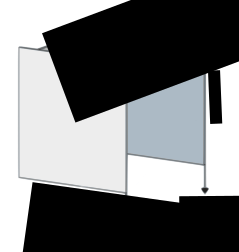
\includegraphics[width=0.8\textwidth]{IsoviewOfPantsModel}
%\caption{Схема нагружения модельных стенок}
%\label{IsoviewOfPantsModel}
%\end{figure}


Уровень нагружения оценивался по величинам касательных напряжений. Касательные напряжения в пластине при чистом сдвиге равны

\begin{equation}
\tau=\frac{3}{2}\cdot\frac{Q}{bh}
\end{equation}
Критические по устойчивости касательные напряжения в пластине при чистом сдвиге равны \cite{Volmir}:

\begin{equation}
\tau_\text{кр}=\frac{K}{12}\frac{\pi^2D}{b^2h} = \frac{K}{12}\frac{\pi^2E}{(1-\mu^2)}\left(\frac{h}{b}\right)^2,\, K=5.34 + 4\frac{a}{b},
\end{equation}
где $a$ - размер пластины вдоль направления действия силы, $b$ - размер пластины поперек направления действия силы, $h$ - толщина пластины, $D$ - изгибная жесткость пластины, $E$ - модуль Юнга, $\mu$ - модуль Пуассона материала пластины, $Q$ - приложенная сила.
Допускаемые толщины найдем из условия

\begin{equation}
\tau_\text{кр} \geq \tau \to h \geq \sqrt[3]{\frac{3\cdot12}{2}\frac{Qb\cdot(1-\mu^2)}{k\pi^2E}} 
\end{equation}
Подставляя значения, получим:

\begin{equation}
Q=\frac{8000}{n}\text{кгс},\,a=1300\text{мм},\,b=1009\text{мм},\,\mu=0.3,\,E=7000\frac{\text{кгс}}{\text{мм}^2}
\end{equation}

\begin{equation}
h \geq \sqrt[3]{\frac{18\cdot8000\cdot1000\cdot(1-\mu^2)}{k\pi^2En}} = \frac{5.67}{\sqrt[3]{n}} 
\end{equation}

Таким образом, для случаев $n = 2$ и $n = 4$  были получены минимальные допустимые толщины, 
равные

\begin{equation}
h\geq4.50\text{мм},\,n=2
\end{equation}
\begin{equation}
h\geq2.83\text{мм},\,n=4
\end{equation}
%\subsubsection{Фюзеляжная часть центроплана}

Другим проблемным местом была фюзеляжная часть центроплана. Из-за требований компоновки, а именно интеграции двигателя, центроплан необходимо делать изогнутым (Рис.\ref{fig:centroplan}). Это вносит дополнительные трудности в виде увеличения веса по сравнению с прямым центропланом. Исследованию фюзеляжной части центроплана (выделена серым на Рис.\ref{fig:centroplan}) посвящена глава \ref{chap:SolvingModel}.

\begin{figure}[ht]
\centering
\includegraphics[width=0.6\textwidth]{centroplan}
\caption{Изогнутый центроплан с выделением исследуемой части}
\label{fig:centroplan}
\end{figure}


\section{Рациональные параметры КСС фюзеляжа}
На основе полученных в разделе \ref{sec:creationOfOneModel} данных была проведена оптимизация толщин стенок отсеков и панелей для выполнения требований прочности конструкции. 

\begin{figure}
	\centering
	\def\svgwidth{\textwidth}
	\input{figures/EpureDistributedLoadN1Bottom.pdf_tex}
	\label{fig:epure:loadn1bottom}
	\caption{fig:epure:loadn1bottom}
\end{figure}

\begin{figure}
	\centering
	\def\svgwidth{\textwidth}
	\input{figures/EpureDistributedLoadN1Top.pdf_tex}
	\label{fig:epure:loadn1top}
	\caption{fig:epure:loadn1top}
\end{figure}

\begin{figure}
	\centering
	\def\svgwidth{\textwidth}
	\input{figures/EpureDistributedLoadN2Bottom.pdf_tex}
	\label{fig:epure:loadn2bottom}
	\caption{fig:epure:loadn2bottom}
\end{figure}

\begin{figure}
	\centering
	\def\svgwidth{\textwidth}
	\input{figures/EpureDistributedLoadN2Top.pdf_tex}
	\label{fig:epure:loadn2top}
	\caption{fig:epure:loadn2top}
\end{figure}

\begin{figure}
	\centering
	\def\svgwidth{\textwidth}
	\input{figures/EpureDistributedLoadN12Bottom.pdf_tex}
	\label{fig:epure:loadn12bottom}
	\caption{fig:epure:loadn12bottom}
\end{figure}

\begin{figure}
	\centering
	\def\svgwidth{\textwidth}
	\input{figures/EpureDistributedLoadN12Top.pdf_tex}
	\label{fig:epure:loadn12top}
	\caption{fig:epure:loadn12top}
\end{figure}

\begin{figure}
	\centering
	\def\svgwidth{\textwidth}
	\input{figures/EpureDistributedWeightBottom.pdf_tex}
	\label{fig:epure:loadweightbottom}
	\caption{fig:epure:loadweightbottom}
\end{figure}

\begin{figure}
	\centering
	\def\svgwidth{\textwidth}
	\input{figures/EpureDistributedWeightTop.pdf_tex}
	\label{fig:epure:loadweighttop}
	\caption{fig:epure:loadweighttop}
\end{figure}

%Параметры оптимизированной модели представлены в таблице \ref{tab:paramsOfOptimizedScheme}

%Остальные две главы будут как приложение к этой мощной главе: исследование влияния искривления кессона центроплана на его вес, выбор рациональной КСС.

\tabulinesep = 1mm
\definecolor{lightgray}{gray}{0.9}
\begin{table}[H]
\captionsetup{justification=centering}
\caption{Таблица рациональных параметров}
\begin{tabu}to \linewidth{*2{|X[m c]}|*2{|X[m c]}|}
\hline
Вес фюзеляжа & 618кг & & \\ \hline
Вес крыльев & 1102кг & & \\ \hline
Вес конструкции & 1722кг & & \\ \hline
\end{tabu}
\end{table}
